%%%%%%%%%%%%%%%%%%%%%%%%%%%%%%%%%%%%%%%%%
%%%%%                               %%%%%
%%%%%     SYSTEM IDENTIFICATION     %%%%%
%%%%%                               %%%%%
%%%%%%%%%%%%%%%%%%%%%%%%%%%%%%%%%%%%%%%%%

\begin{frame}[t, c]{}{}
  \begin{minipage}{.48\textwidth}
    \centering
    % 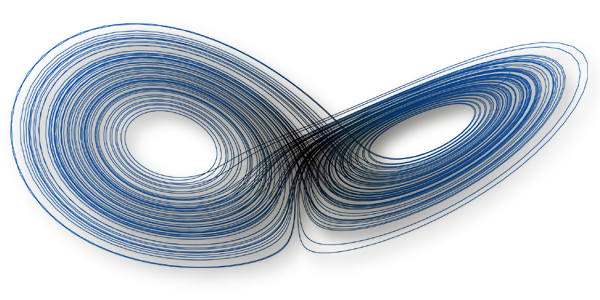
\includegraphics[width=\textwidth]{cover}
    \movie[autostart, loop, width=\textwidth]{
      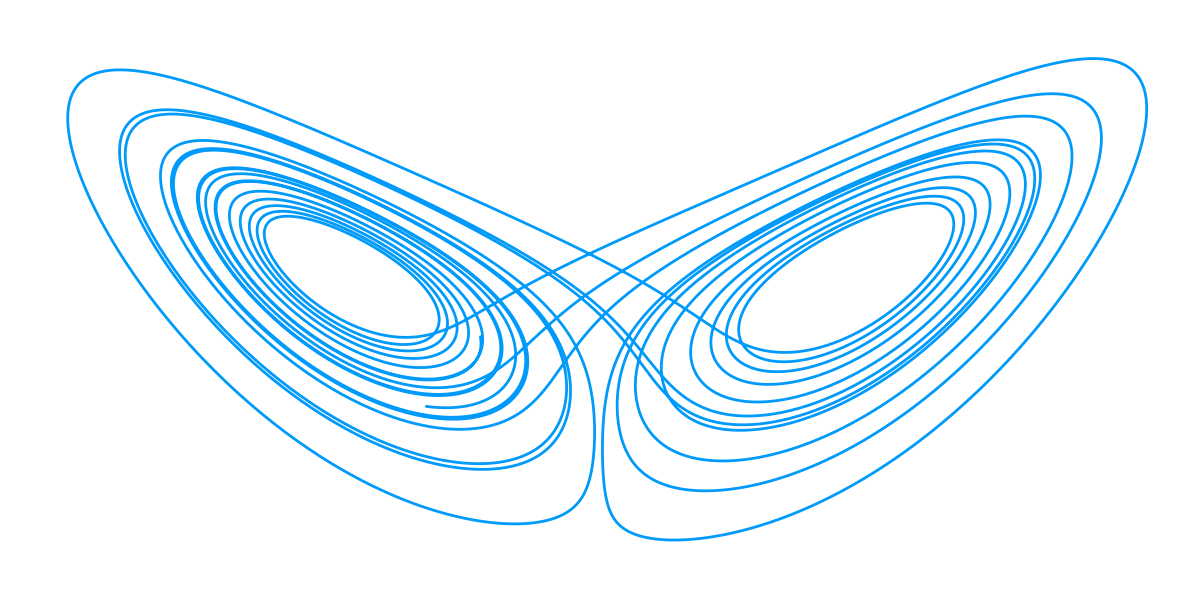
\includegraphics[width=\textwidth]{imgs/lorenz.png}}{imgs/lorenz.wmv}
  \end{minipage}%
  \hfill
  \begin{minipage}{.48\textwidth}
    \centering
    {
      \Large\textbf{Part III}
    }
    
    \bigskip
    
    \rule{\textwidth}{0.001\textwidth}
    
    \bigskip
    
    {
      \large
      \textbf{Sparse Identification of Nonlinear Dynamics}
    }
    
    \medskip
    
    \begin{itemize}
    \item Problem formulation:
      % 
      \begin{itemize}
      \item[\(	\hookrightarrow	\)] Physical constraints
      \item[\(	\hookrightarrow	\)] Optimization problem
      \item[\(	\hookrightarrow	\)] Greedy algorithms and convex relaxations
      \end{itemize}
      
      \medskip
      
    \item Application to the chaotic thermosyphon:
      \begin{itemize}
      \item[\(	\hookrightarrow	\)] A Lorenz-like system
      \item[\(	\hookrightarrow	\)] Cross-validations
      \end{itemize}
      
    \end{itemize}
    
  \end{minipage}
\end{frame}

\begin{frame}[t, c]{Identifying a dynamical system}{Overview}
  \begin{minipage}{.48\textwidth}
    \begin{block}{}
      \centering
      \textbf{Sparse Identification of Nonlinear Dynamics}
    \end{block}
    
    \medskip
    
    \begin{itemize}
    \item \textbf{Aim:} Identify a low-order nonlinear dynamical system
      \begin{itemize}
      \item[\(	\hookrightarrow	\)] Inherently interpretable set of ODE.
      \item[\(	\hookrightarrow	\)] Fast evaluation for forecasting.
      \end{itemize}
      
      \medskip
      
    \item \textbf{How:} Sparse least-squares regression
      \begin{itemize}
      \item[\(	\hookrightarrow	\)] Constraints for physical consistency.
      \item[\(	\hookrightarrow	\)] Greedy algorithms/convex relaxations.
      \end{itemize}
    \end{itemize}
  \end{minipage}%
  \hfill
  \begin{minipage}{.48\textwidth}
    \centering
    \includegraphics[width=\textwidth]{physics_machine_learning}
  \end{minipage}
  
  \vspace{1cm}
\end{frame}

\begin{frame}[t, c]{Sparse Identification of Nonlinear Dynamics}{Overview}
  \begin{minipage}{.48\textwidth}
    \begin{itemize}
    \item Brunton \emph{et al.}, \emph{Proc. Natl. Acad. Sci. U.S.A.}, 2015.
      
      \medskip
      
    \item Relies on a dictionnary of pre-defined functions and sparsity-promoting regression.
      
      \medskip
      
    \item Quite promissing and versatile framework.
    \end{itemize}
  \end{minipage}%
  \hfill
  \begin{minipage}{.48\textwidth}
    \centering
    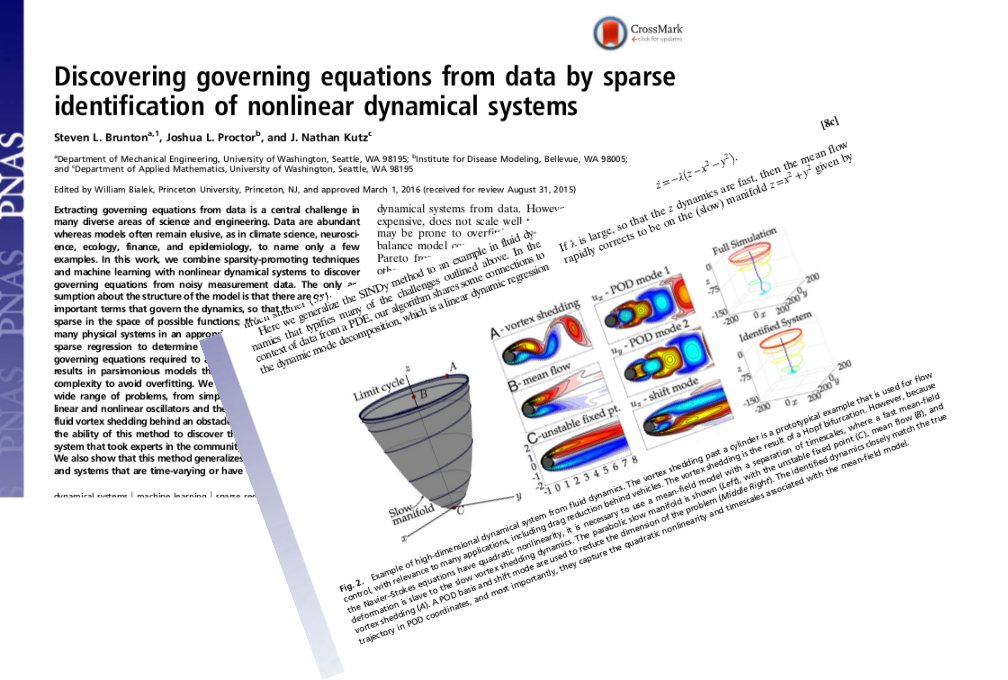
\includegraphics[width=\textwidth]{sindy_paper}
  \end{minipage}
  
  \vspace{1cm}
\end{frame}

\begin{frame}[t, c]{Sparse Identification of Nonlinear Dynamics}{A combinatorial problem}
  \begin{minipage}{.48\textwidth}
    \centering
    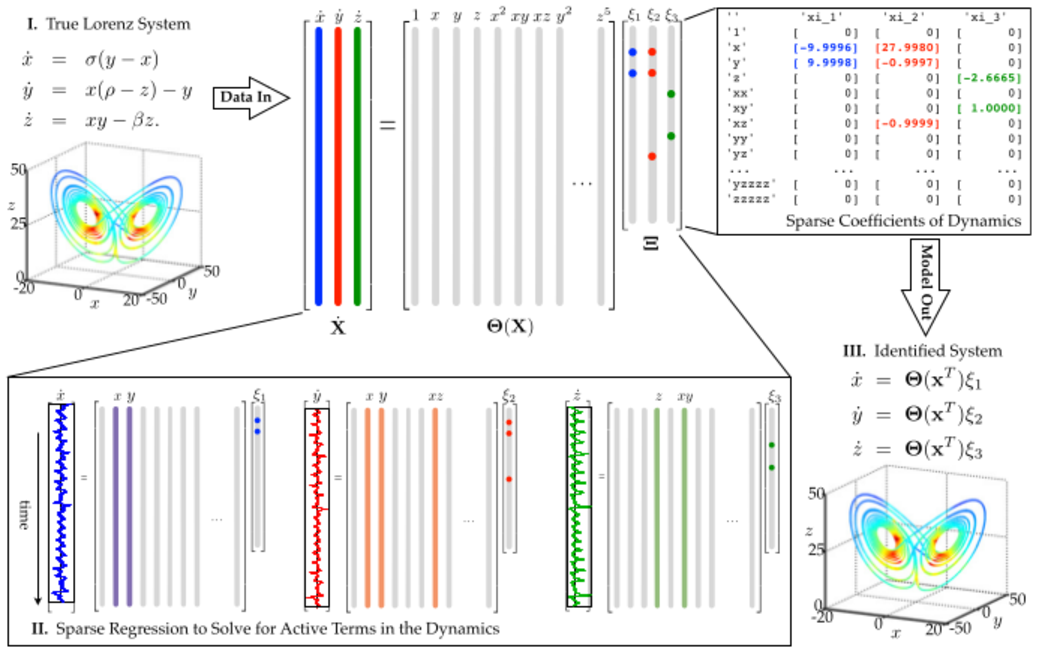
\includegraphics[width=\textwidth]{sparse_identification}
  \end{minipage}%
  \hfill
  \begin{minipage}{.48\textwidth}
    \begin{itemize}
    \item Given \(	\boldsymbol{\Uptheta}(\bm{x})	\), one aims to solve
      % 
      \[
        \begin{aligned}
          \minimize_{\boldsymbol{\upxi}} & \text{card }(\boldsymbol{\upxi}) \\
          \subjecto & \| \boldsymbol{\Uptheta}(\bm{x}) \boldsymbol{\upxi} - \dot{\bm{x}} \|_2^2 \leq \sigma.
        \end{aligned}
      \]
      
    \item Rapidly intractable combinatorial problem.
      
      \medskip
      
    \item Convex relaxation and/or greedy algorithms needed.
    \end{itemize}
  \end{minipage}
  
  \vspace{1cm}
\end{frame}

\begin{frame}[t, c]{Sparse Identification of Nonlinear Dynamics}{Problem formulation: general form}
  \begin{itemize}
  \item Navier-Stokes are nonlinear PDEs with quadratic nonlinearities so the dictionnary is chosen as
    % 
    \[
      \boldsymbol{\Uptheta}(\bm{x}) = \begin{bmatrix} 1 & x & y & z & x^2 & xy & xz & y^2 & yz & z^2 \end{bmatrix}.
    \]
    
    \medskip
    
  \item The yet-unknown model takes the following general form
    % 
    \[
      \begin{aligned}
        \dot{x} & = a_0 + a_1 x + a_2 y + a_3 z + a_4 x^2 + a_5 xy + a_6 xz + a_7 y^2 + a_8 yz + a_9 z^2 \\
        \dot{y} & = b_0 + b_1 x + b_2 y + b_3 z + b_4 x^2 + b_5 xy + b_6 xz + b_7 y^2 + b_8 yz + b_9 z^2 \\
        \dot{z} & = c_0 + c_1 x + c_2 y + c_3 z + c_4 x^2 + c_5 xy + c_6 xz + c_7 y^2 + c_8 yz + c_9 z^2
      \end{aligned}
    \]
    
    \medskip
    
  \item Up to 30 coefficients need to be identified using our training data.
  \end{itemize}
  
  \vspace{1cm}
\end{frame}

\begin{frame}[t, c]{Sparse Identification of Nonlinear Dynamics}{Problem formulation: equivariant system}
  \begin{minipage}{.68\textwidth}
    \begin{itemize}
    \item System is equivariant w.r.t.\ to the transformation \( (x, y, z) \mapsto (-x, -y, z) \).
      We thus have
      % 
      \[
        \gamma \cdot \dot{\bm{x}} = \bm{f}\left( \gamma \cdot \bm{x} \right)
      \]
      % 
      with \( \gamma \) the matrix representation of the flip operator.
      
      \smallskip
      
    \item The yet-unknown model reduces to
      % 
      \[
        \begin{aligned}
          \dot{x} & = a_0 x + a_1 y + a_2 xz + a_3 yz \\
          \dot{y} & = b_0 x + b_1 y + b_2 xz + b_3 yz \\
          \dot{z} & = c_0 + c_1 z + c_2 x^2 + c_3 xy + c_4 y^2 + c_5 z^2
        \end{aligned}
      \]
      
      \smallskip
      
    \item Only 14 terms need to be actually identified.
      
    \end{itemize}
  \end{minipage}%
  \hfill
  \begin{minipage}{.28\textwidth}
    \centering
    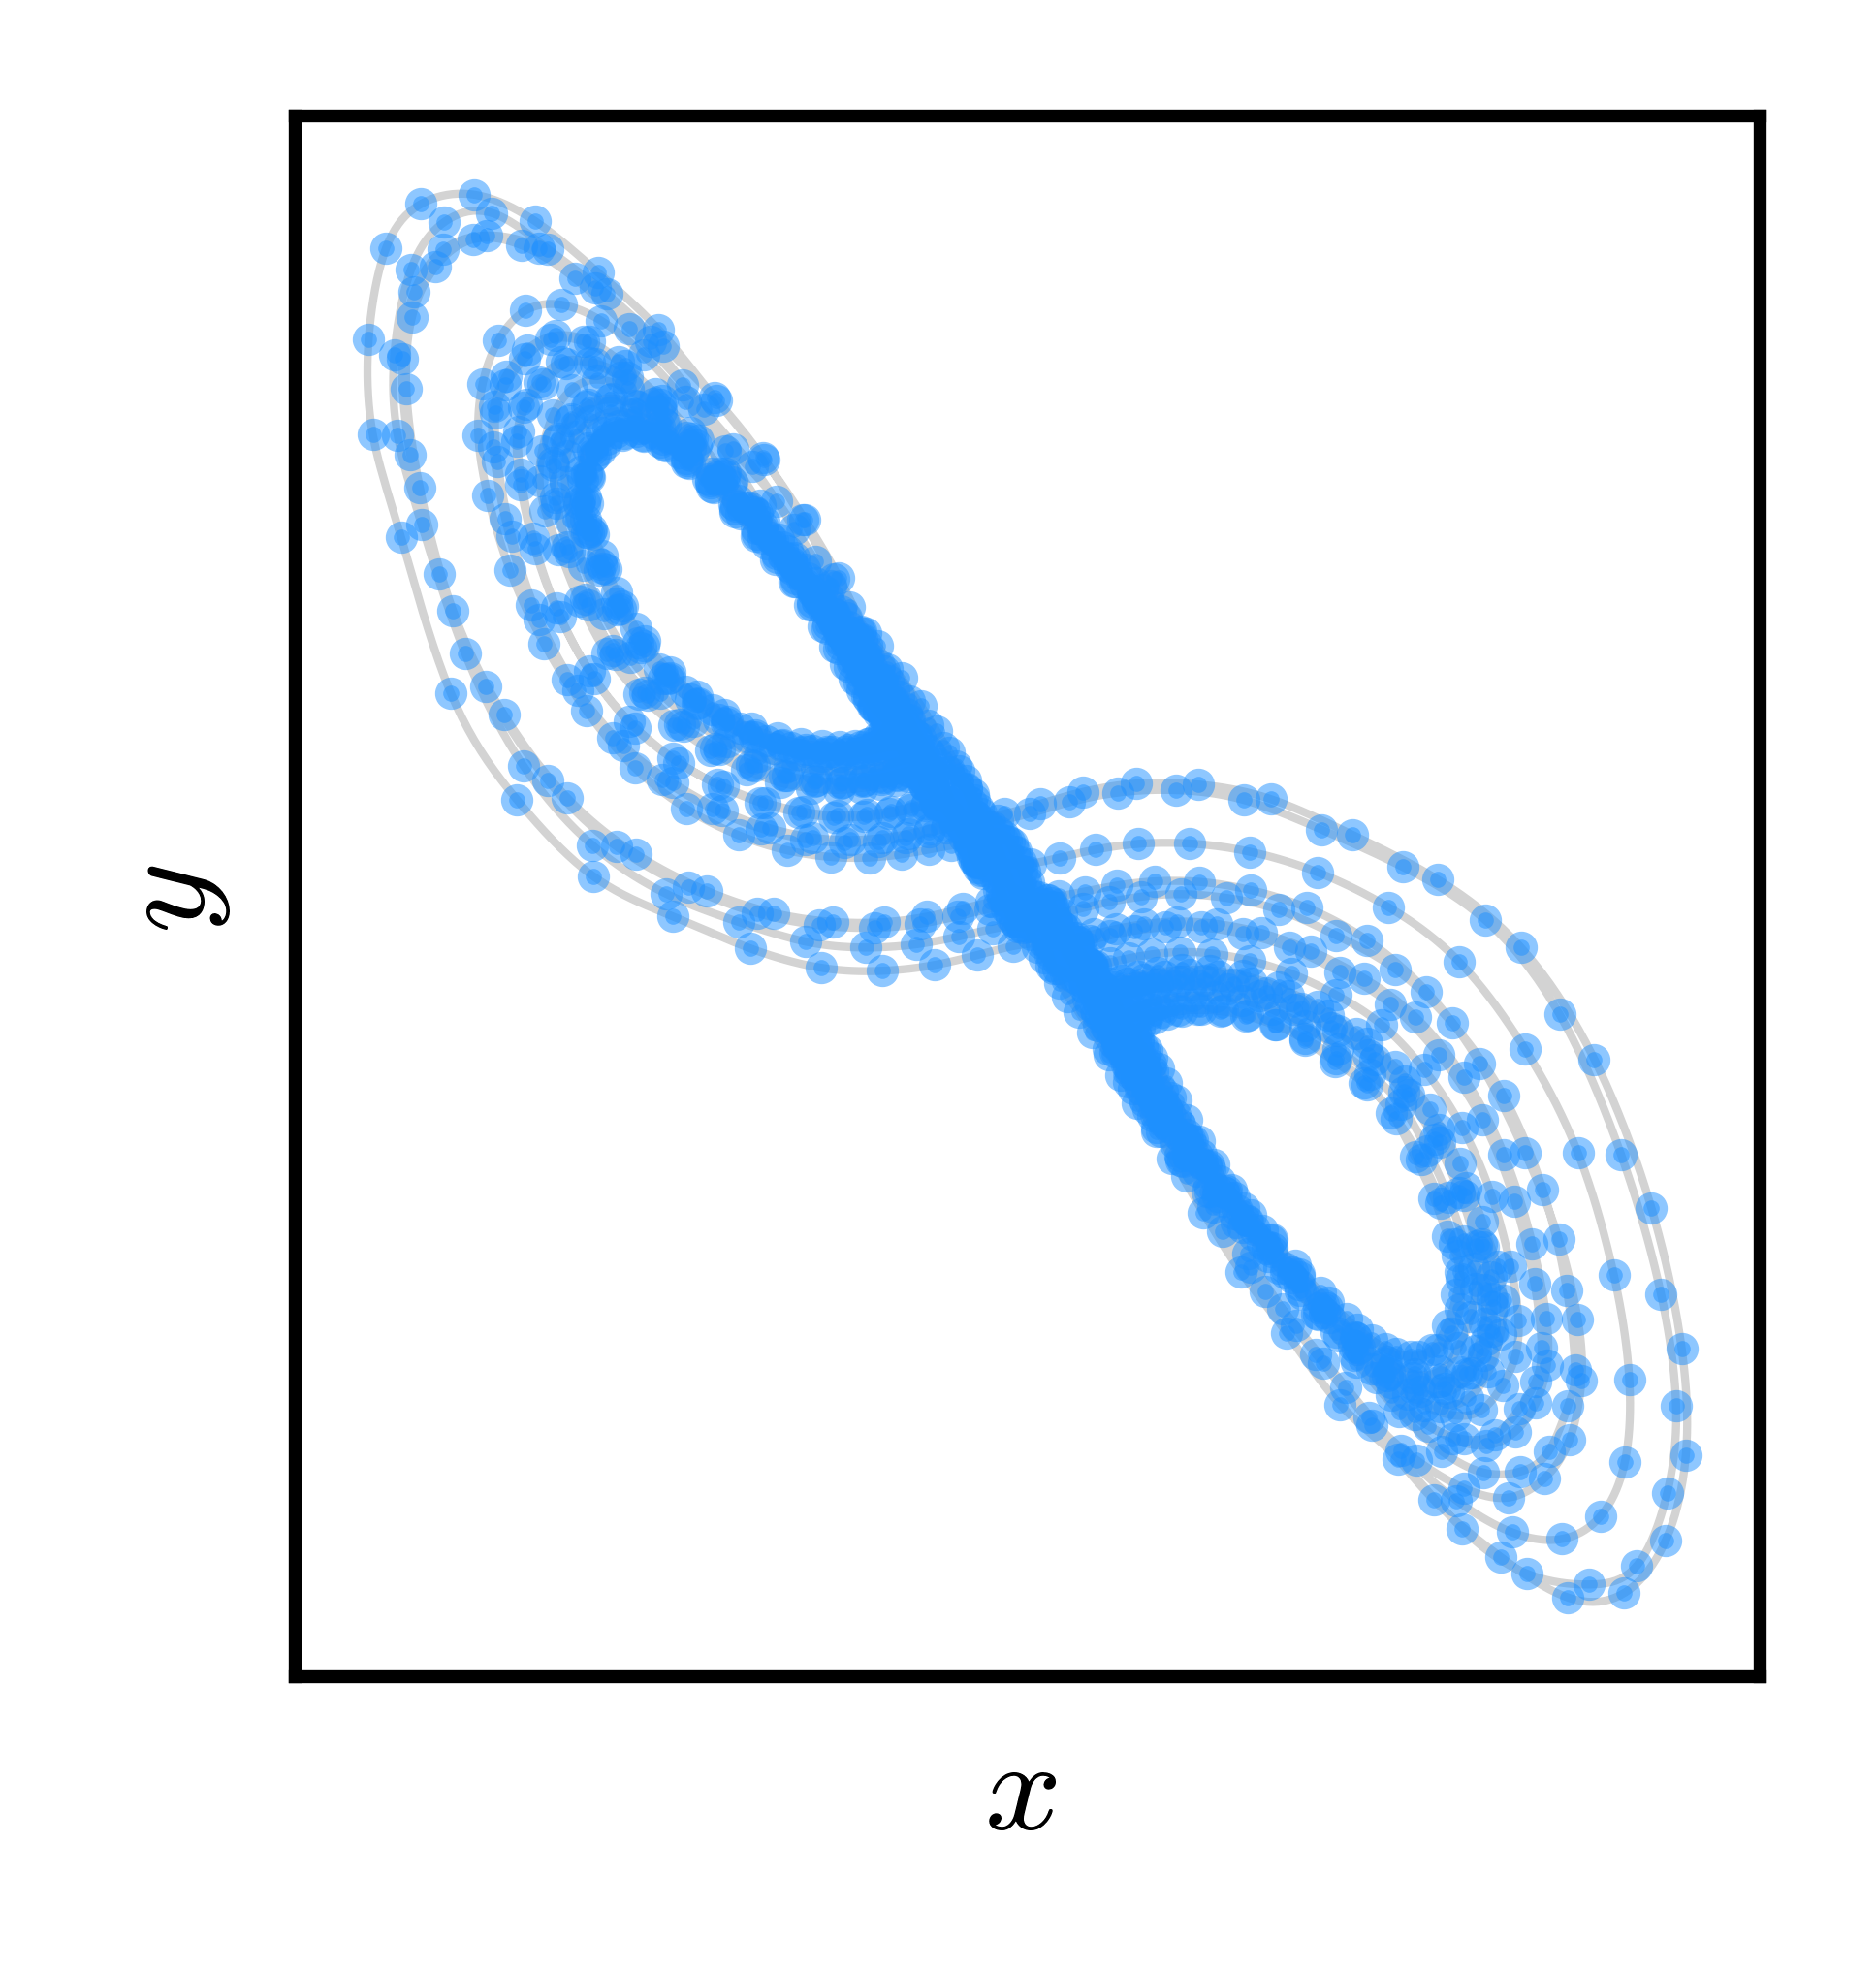
\includegraphics[width=\textwidth]{flip_symmetry}
  \end{minipage}
  
  \vspace{1cm}
\end{frame}

\begin{frame}[t, c]{Sparse Identification of Nonlinear Dynamics}{Problem formulation: dissipative system}
  \begin{minipage}{.28\textwidth}
    \centering
    \movie[width=\textwidth]{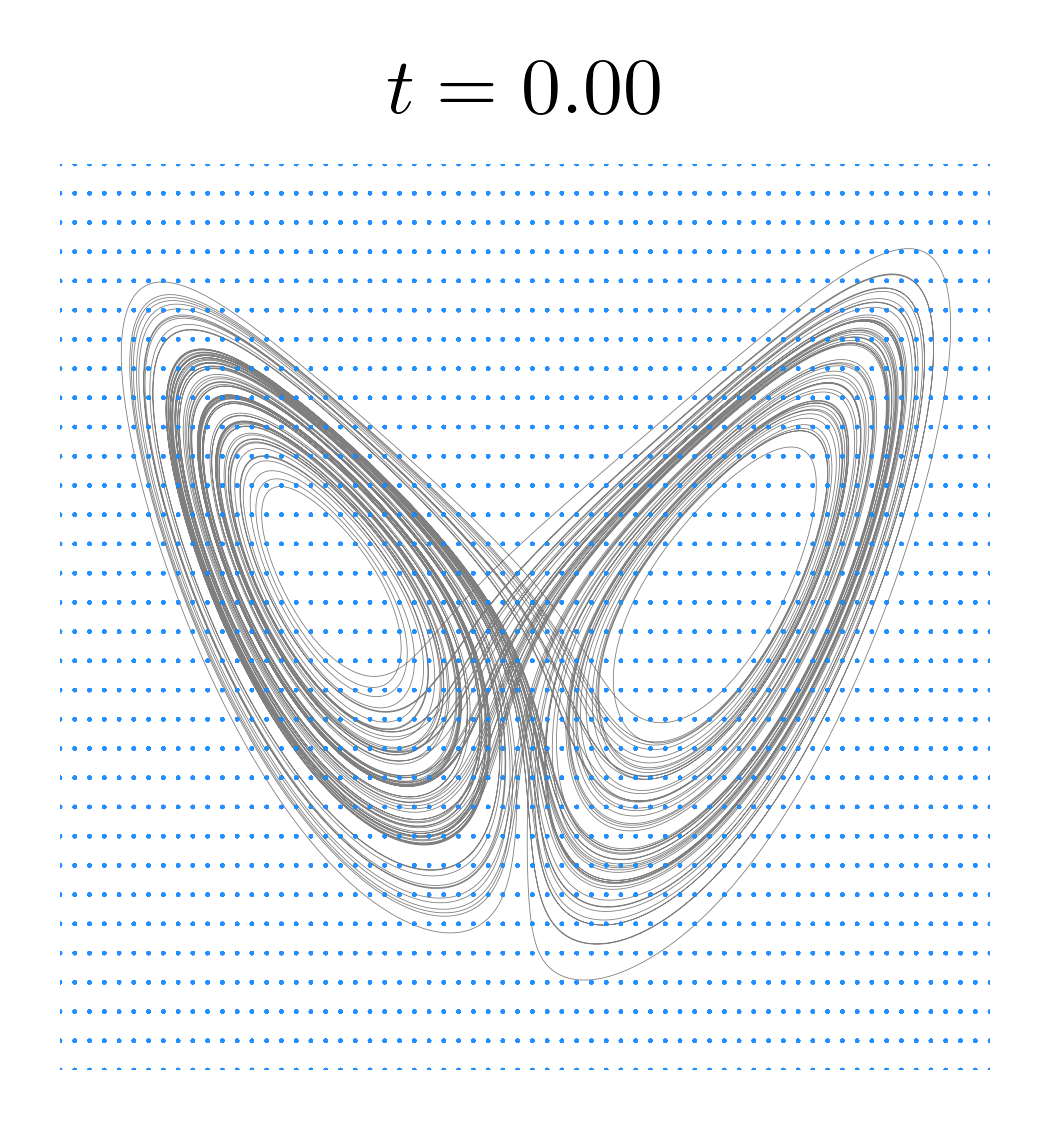
\includegraphics[width=\textwidth]{dissipative_system}}{imgs/dissipative_system.mp4}
  \end{minipage}%
  \hfill
  \begin{minipage}{.68\textwidth}
    \begin{itemize}
    \item The system \( \dot{\bm{x}} = \bm{f}(\bm{x}) \) is \underline{dissipative}, thus
      % 
      \[
        \nabla \cdot \bm{f}(\bm{x}) < 0 \quad \forall \bm{x}.
      \]
      
      \medskip
      
    \item It yields to the following constraints
      % 
      \[
        \begin{aligned}
          a_0 + b_1 + c_1 & < 0, \\
          a_2 + b_3 + 2c_5 & = 0.
        \end{aligned}
      \]
      
      \medskip
      
    \item All three equations are coupled by these constraints and need to be identified jointly.
    \end{itemize}
  \end{minipage}
  
  \vspace{1cm}
\end{frame}

\begin{frame}[t, c]{Sparse Identification of Nonlinear Dynamics}{Problem formulation: energy-preserving quadratic nonlinearities}
  \begin{minipage}{.58\textwidth}
    \begin{itemize}
    \item Quadratic nonlinearities in Navier-Stokes are energy-preserving.
      
      \medskip
      
    \item For our system, energy equation would read
      % 
      \[
        \dot{E} = c_0 z + a_0 x^2 + b_1 y^2 + c_1 z^2 + (a_1 + b_0) xy.
      \]
      
    \item The following constraints need to be satistifed
      % 
      \[
        \begin{aligned}
          & b_3 + c_4 = 0, \quad a_2 + c_2 = 0 \\
          & a_3 + b_2 + c_3 = 0.
        \end{aligned}
      \]
    \end{itemize}
  \end{minipage}%
  \hfill
  \begin{minipage}{.38\textwidth}
    \begin{equation}
      \begin{aligned}
        \textrm{State equation : } & \dot{\bm{x}} = \bm{b} + \bm{Ax} + \mathcal{Q}(\bm{x}) \\
        \textrm{Energy : } & E = \frac{1}{2} \bm{x}^T \bm{x} \\
        \textrm{Energy equation : } & \dot{E} = \bm{x}^T \left( \bm{b} + \bm{Ax} \right)
      \end{aligned}
      \notag
    \end{equation}
  \end{minipage}
  
  \vspace{1cm}
\end{frame}

\begin{frame}[t, c]{Sparse Identification of Nonlinear Dynamics}{Final problem}
  \begin{minipage}{.58\textwidth}
    \begin{overprint}
      \onslide<1>
      Our optimization problem finally takes the following form
      % 
      \[
        \begin{aligned}
          \minimize_{\boldsymbol{\upxi}} & \text{card}(\boldsymbol{\upxi}) \\
          \subjecto & \| \boldsymbol{\Uptheta}(\bm{x}) \boldsymbol{\upxi} - \dot{\bm{x}} \|_2^2 < \sigma \\
          & \bm{C} \boldsymbol{\upxi} = 0 \\
          & \bm{D} \boldsymbol{\upxi} < 0.
        \end{aligned}
      \]
      % 
      with \( \boldsymbol{\upxi} = \begin{bmatrix} \boldsymbol{\upxi}_x & \boldsymbol{\upxi}_y & \boldsymbol{\upxi}_z \end{bmatrix}^T \) the vector of unknown coefficients.
      
      \onslide<2>
      In practice, this combinatorial problem is approximated by a convex relaxation, e.g.
      % 
      \[
        \begin{aligned}
          \minimize_{\boldsymbol{\upxi}} & \| \boldsymbol{\Uptheta}(\bm{x}) \boldsymbol{\upxi} - \dot{\bm{x}} \|_2^2 + \lambda R(\boldsymbol{\upxi}) \\
          \subjecto & \bm{C} \boldsymbol{\upxi} = 0 \\
          & \bm{D} \boldsymbol{\upxi} < 0,
        \end{aligned}
      \]
      % 
      with \( R(\bm{x}) \) some sparsity promoting heuristic.
      Here, we chose \( R(\bm{x}) = \| \boldsymbol{\upxi} \|_2^2 \) (i.e.\ Thikonov regularization).
    \end{overprint}
  \end{minipage}%
  \hfill
  \begin{minipage}{.38\textwidth}
    \centering
    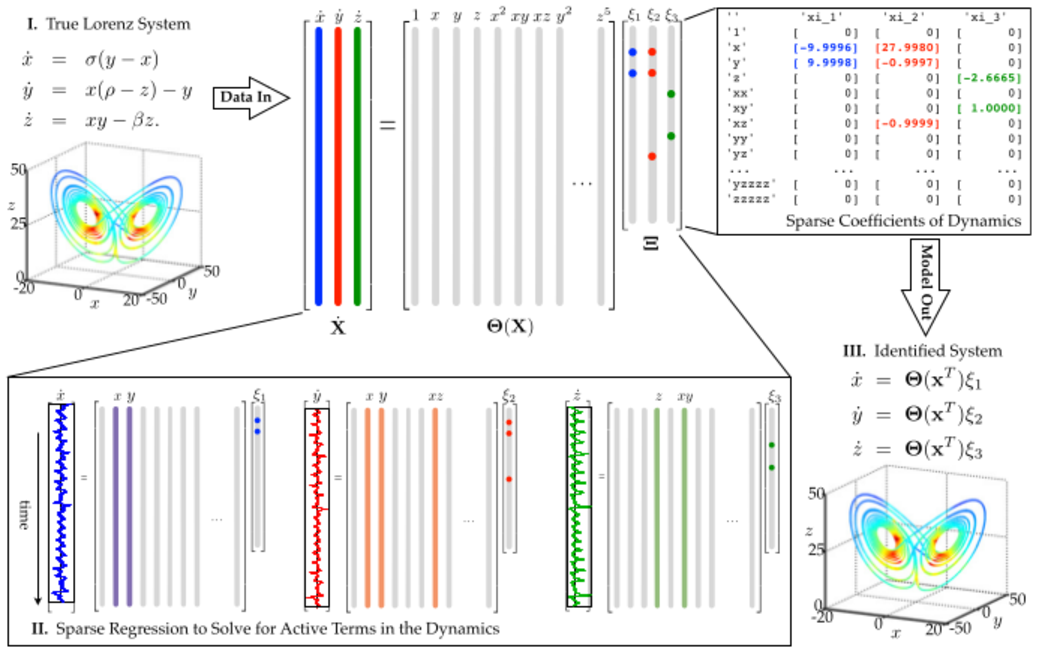
\includegraphics[width=\textwidth]{sparse_identification}
  \end{minipage}
  
  \vspace{1cm}
\end{frame}

\begin{frame}[t, c]{Sparse Identification of Nonlinear Dynamics}{Identifying the model}
  \begin{minipage}{.68\textwidth}
    \begin{itemize}
    \item Our dataset spans \( 500 \tau \) time-units.
      A sequence of \( 400 \tau \) is used for training while the remaining \( 100 \tau \) are used for testing.
      
      \medskip
      
    \item The optimization problem is implemented using the python bindings of \texttt{cvxopt}.
      
      \medskip
      
    \item Model selection is based on the ability of the identified system to reproduce the second-order statistics of the true system.
    \end{itemize}
  \end{minipage}%
  \hfill
  \begin{minipage}{.28\textwidth}
    \centering
    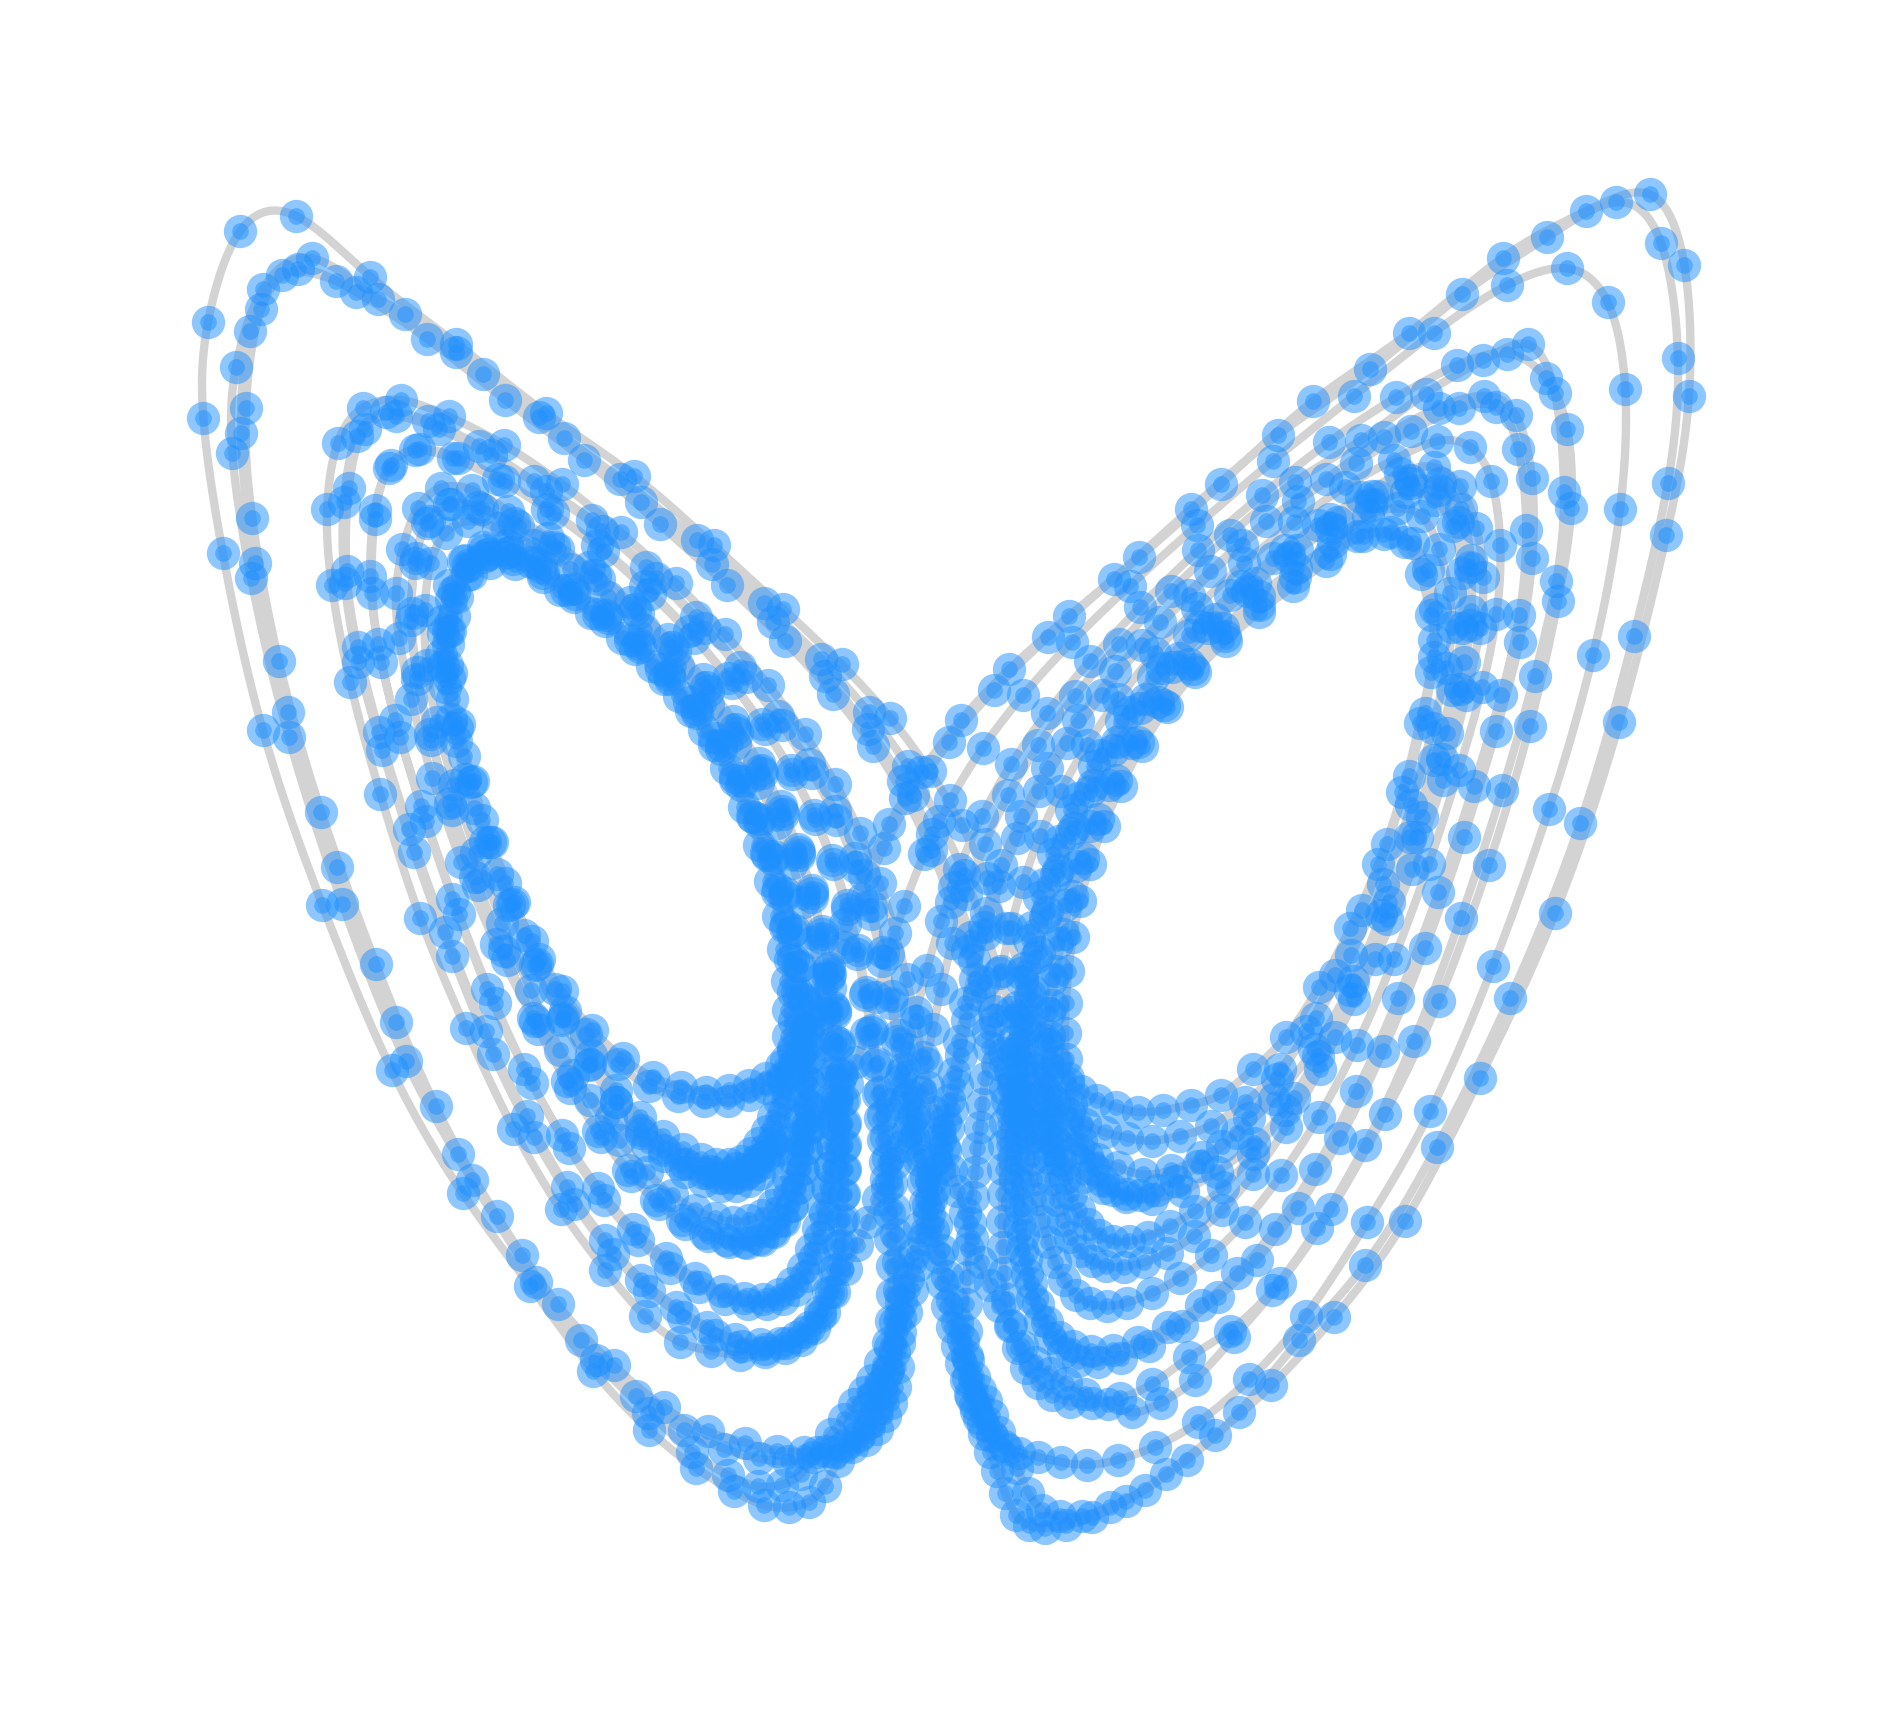
\includegraphics[width=\textwidth]{latent_space}
  \end{minipage}
  
  \vspace{1cm}
\end{frame}

\begin{frame}[t, c]{Sparse Identification of Nonlinear Dynamics}{Identified systems and model selection}
  \centering
  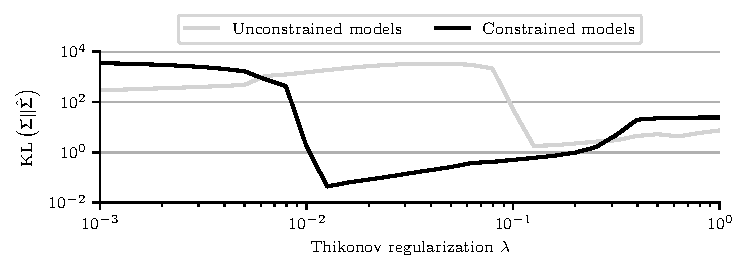
\includegraphics[width=.9\textwidth]{KL_divergence_model_selection}
  
  {\small
    \[
      \textrm{KL}(\bm{A} \vert \bm{B}) = \frac{1}{2} \left( \textrm{Tr}(\bm{B}^{-1}\bm{A}) - n + \ln \frac{\vert \bm{B} \vert}{\vert \bm{A} \vert} \right)
    \]
  }
  
  \vspace{1cm}
\end{frame}

\begin{frame}[t, c]{Sparse Identification of Nonlinear Dynamics}{Selected model}
  \begin{minipage}{.68\textwidth}
    
    \begin{block}{\centering \textbf{Selected model}}
      \[
        \begin{aligned}
          \dot{x} & = -76.08 x + 88.39 y \\
          \dot{y} & = 20.76 x - 4.19 y - 41.49 xz \\
          \dot{z} & = -43.67 - 17.31 z + 41.49 xy.
        \end{aligned}
      \]
    \end{block}
    
    \medskip
    
    \begin{itemize}
    \item \underline{Lorenz-like} system satisfying all of the physical constraints by design.
      
      \medskip
      
    \item Every single term can be intepreted and associated to a particular physical mechanism.
    \end{itemize}
  \end{minipage}%
  \hfill
  \begin{minipage}{.28\textwidth}
    \centering
    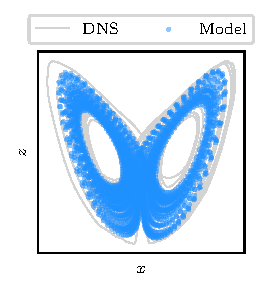
\includegraphics[width=\textwidth]{attractor_comparison}
  \end{minipage}
  
  \vspace{1cm}
\end{frame}

\begin{frame}[t, c]{Sparse Identification of Nonlinear Dynamics}{Selected model}
  \centering
  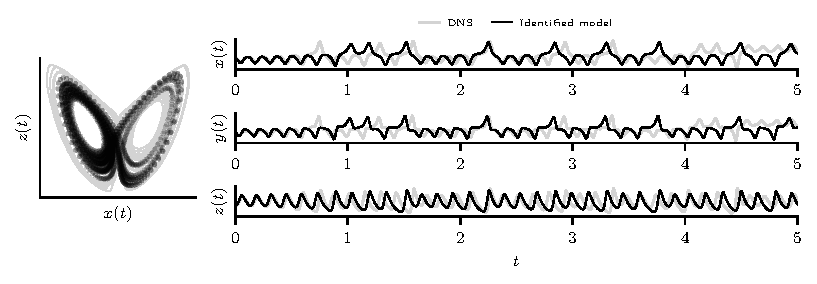
\includegraphics[width=.9\textwidth]{attractor_comparison_bis}
\end{frame}


% \begin{frame}[t, c]{Sparse Identification of Nonlinear Dynamics}{Physical mechanisms at play}
%   \centering
  
%   \begin{overprint}
%     \onslide<1>
%     \centering
%     \includegraphics[height=.7\textheight]{high_level_description}
    
%     \onslide<2>
%     \centering
%     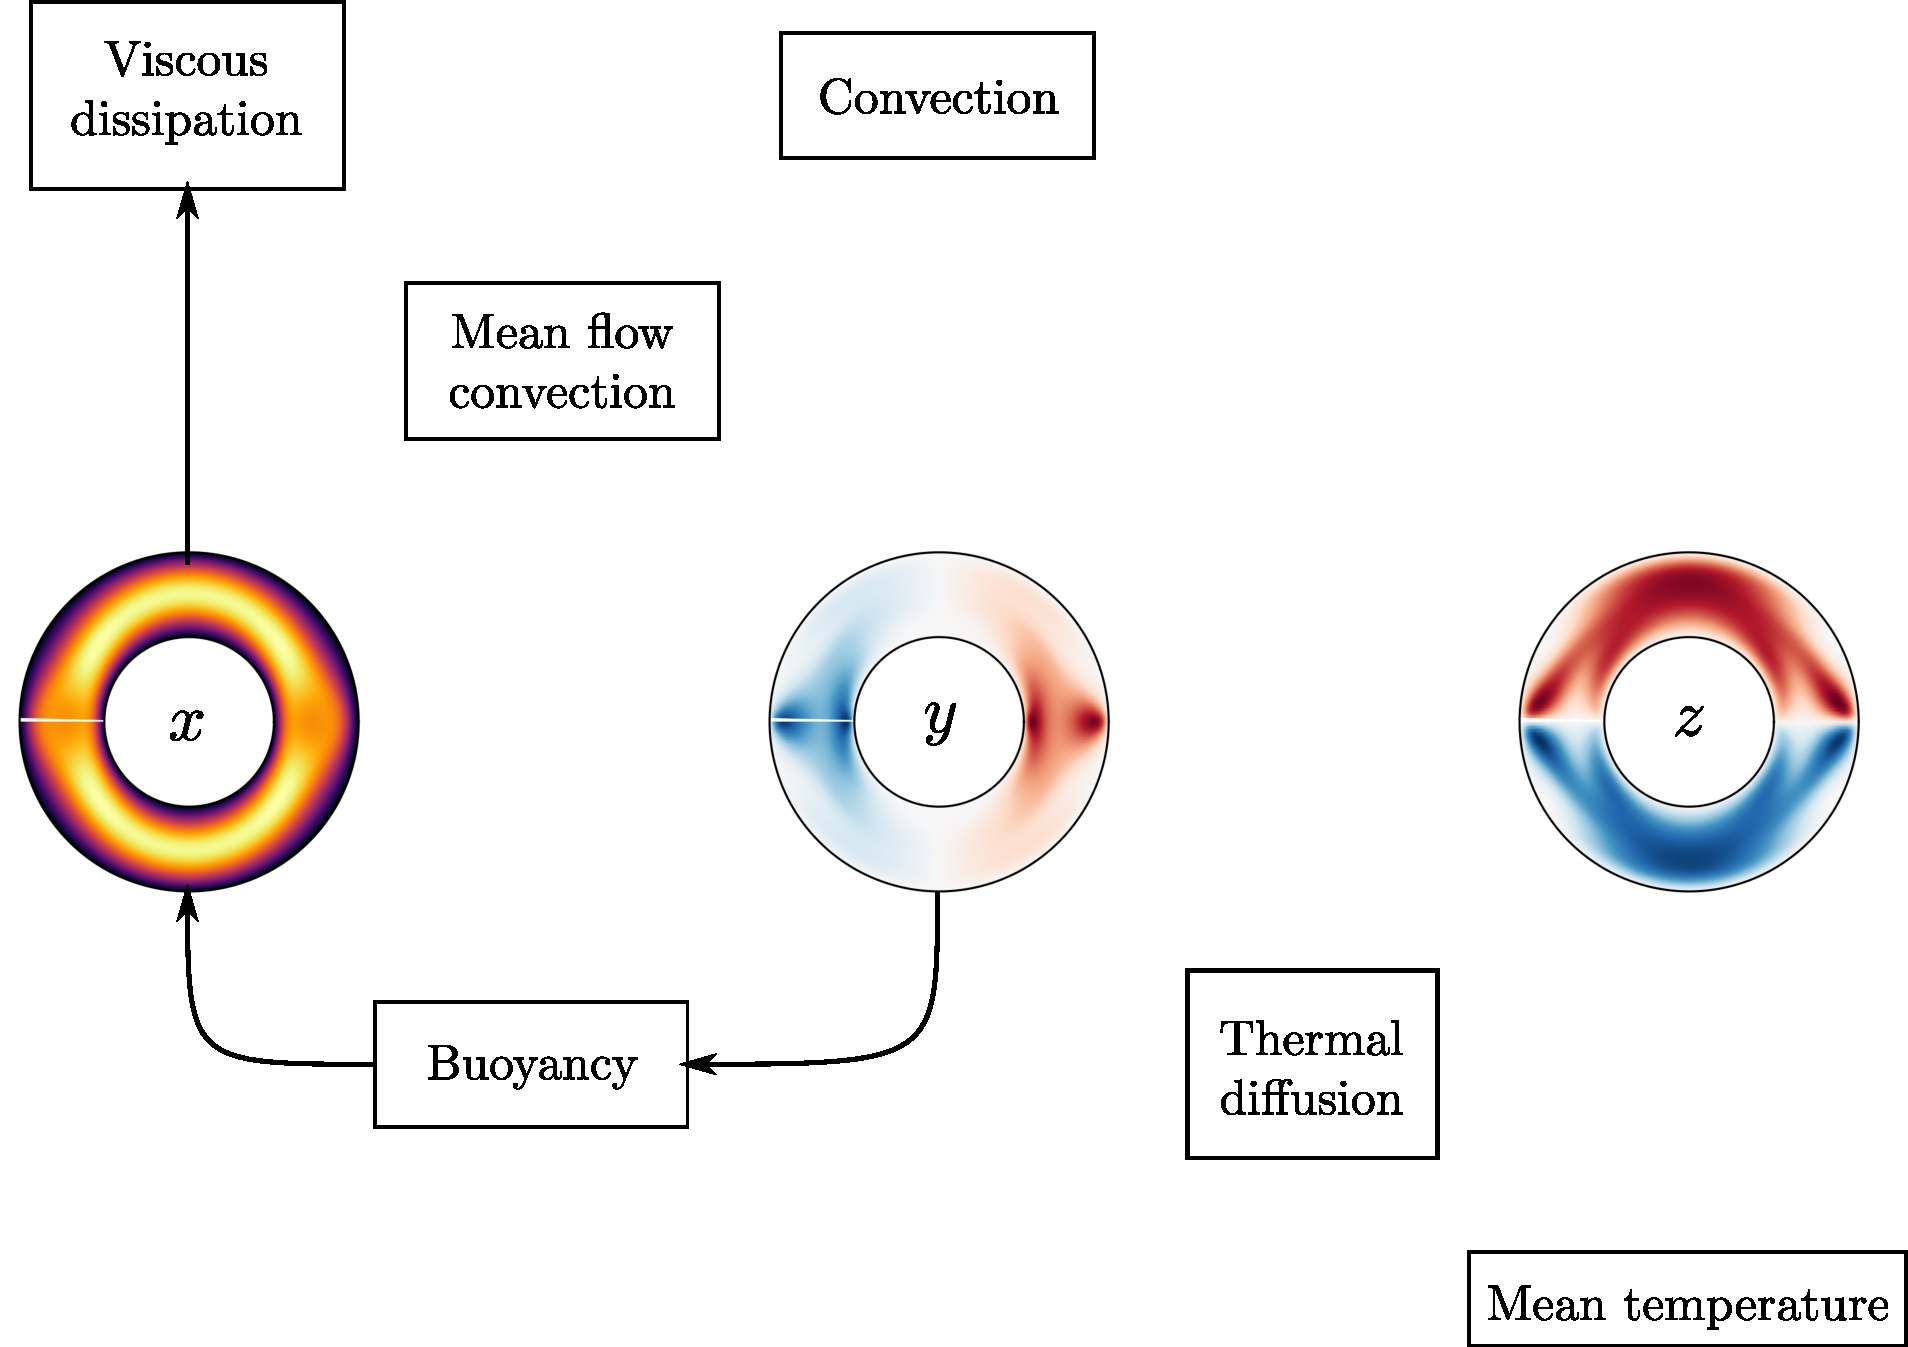
\includegraphics[height=.7\textheight]{high_level_description_x}
    
%     \onslide<3>
%     \centering
%     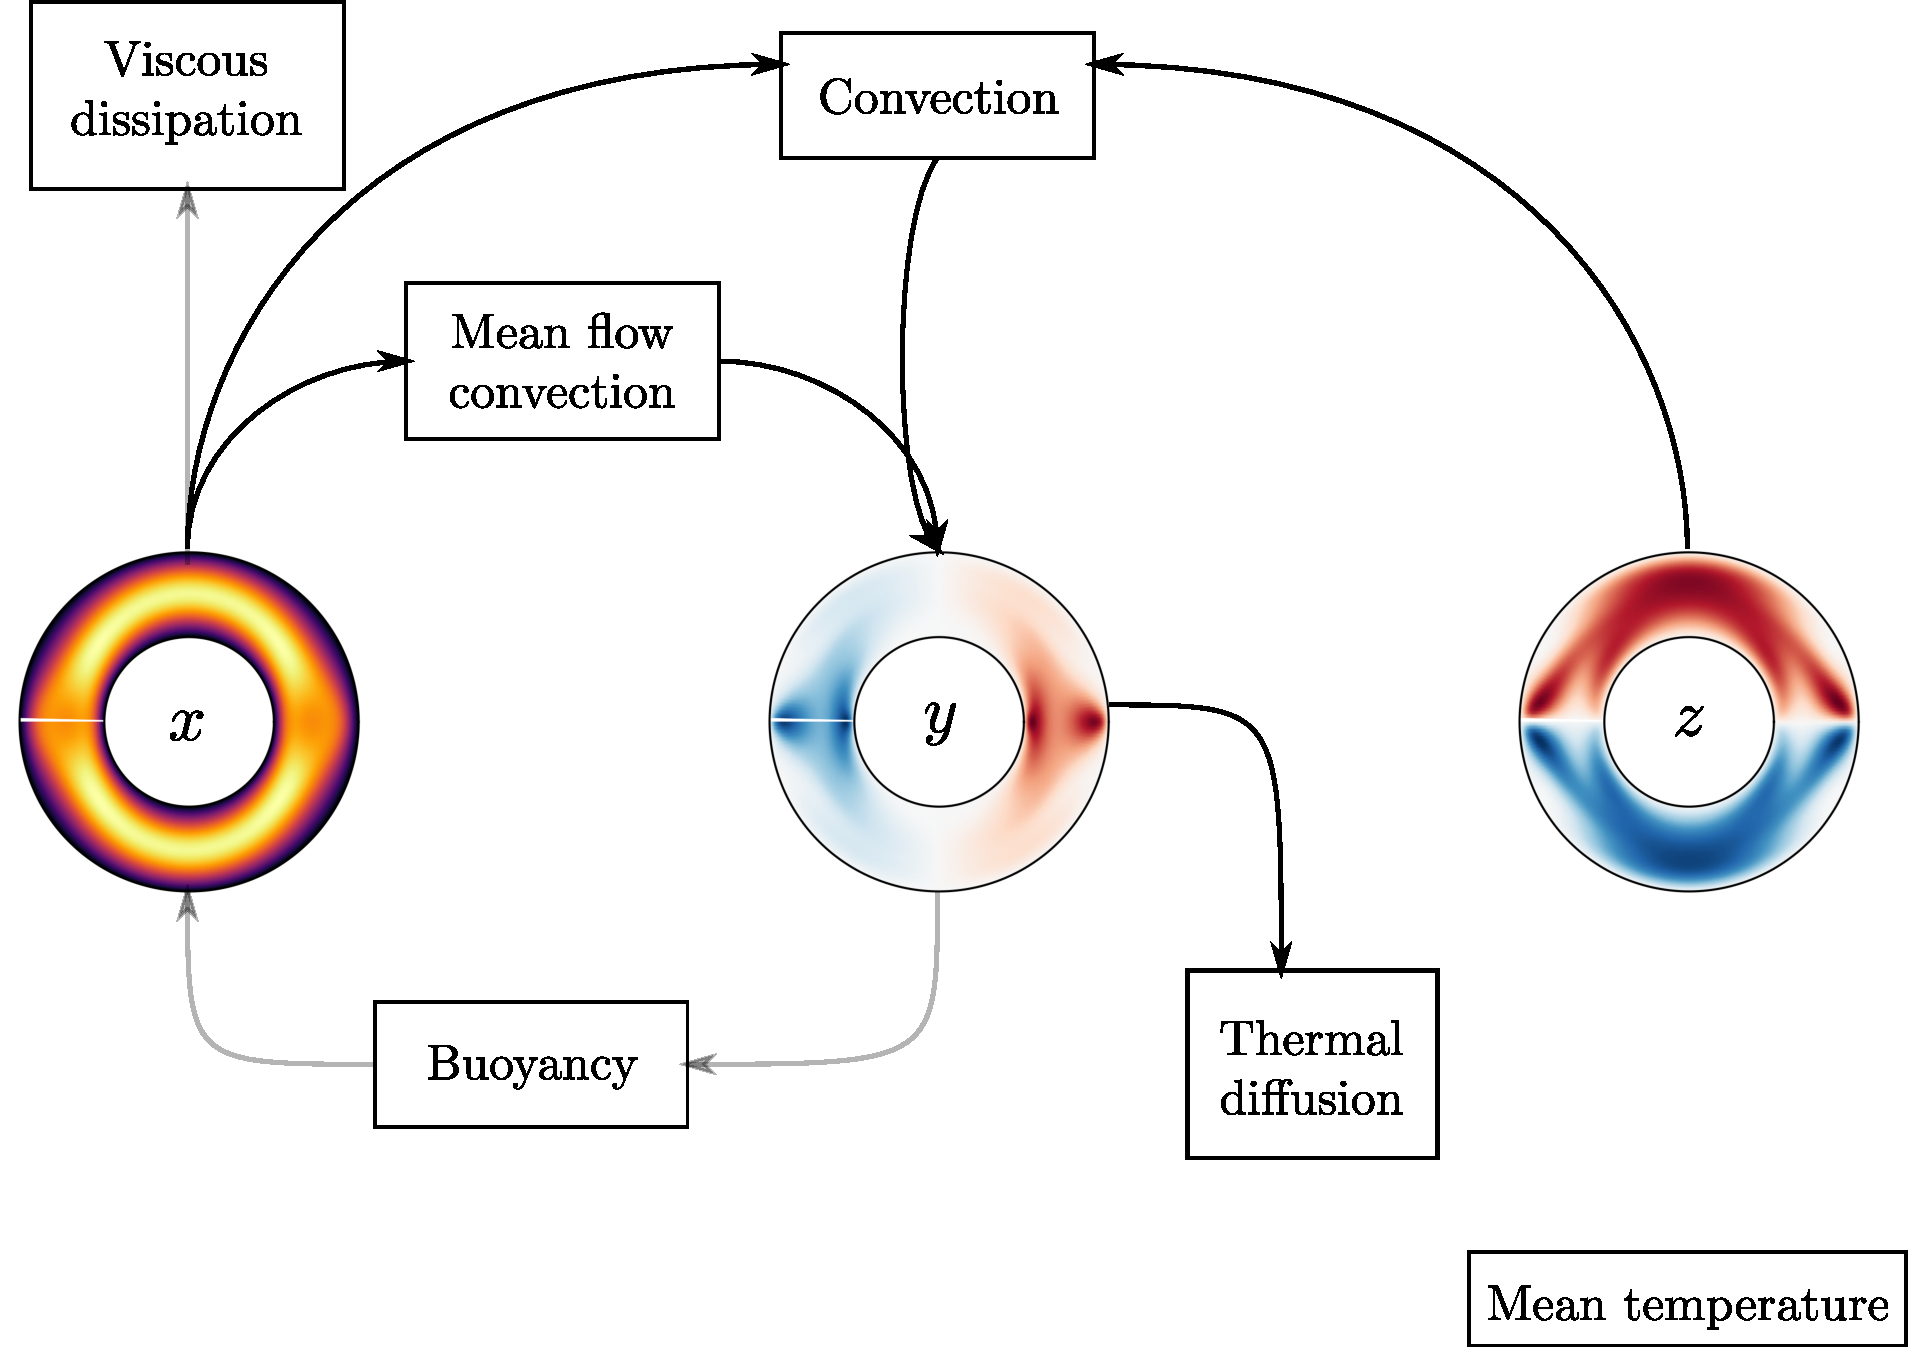
\includegraphics[height=.7\textheight]{high_level_description_y}
    
%     \onslide<4>
%     \centering
%     \includegraphics[height=.7\textheight]{high_level_description_z}
    
%   \end{overprint}
  
%   \vspace{1cm}
% \end{frame}


\begin{frame}[t, c]{Sparse Identification of Nonlinear Dynamics}{Comparing the statistical properties}
  \begin{minipage}{.48\textwidth}
    \centering
    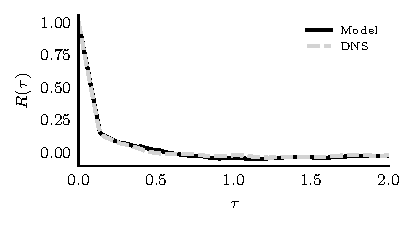
\includegraphics[width=.95\textwidth]{autocorrelation_function_comparison}

  \end{minipage}%
  \hfill
  \begin{minipage}{.48\textwidth}
    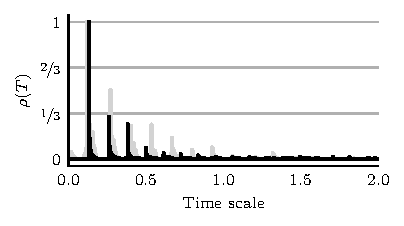
\includegraphics[width=.95\textwidth]{time_scale_distribution_comparison}
  \end{minipage}

  \bigskip
  
  \centering
  The model accurately captures the dynamical properties of the switches.
  
  \vspace{1cm}
\end{frame}

\begin{frame}[t, c]{Sparse Identification of Nonlinear Dynamics}{Comparing the statistical properties}

  \begin{center}
    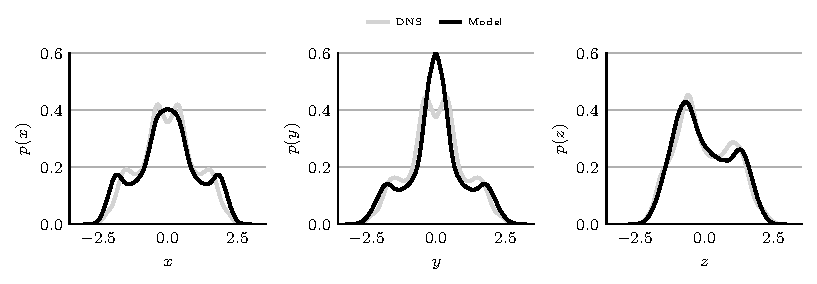
\includegraphics[width=.8\textwidth]{probability_density_functions}
  \end{center}

  \medskip

  Overall agreements regarding the probability density functions albeit there is a small (yet unexplained) mismatch in the center.
  \vspace{1cm}
\end{frame}

% \begin{frame}[t, c]{Sparse Identification of Nonlinear Dynamics}{Quantitative comparison with the true system}
%   \begin{minipage}{.28\textwidth}
%     \begin{overprint}
%       \onslide<1>
%       \centering
%       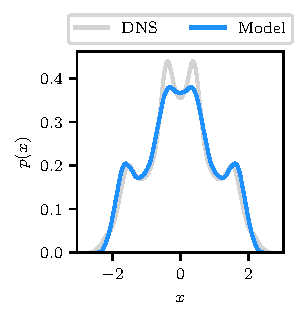
\includegraphics[width=\textwidth]{pdf_comparison_x}
      
%       \onslide<2>
%       \centering
%       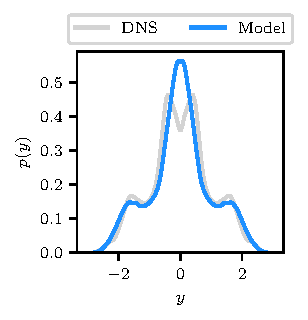
\includegraphics[width=\textwidth]{pdf_comparison_y}
      
%       \onslide<3>
%       \centering
%       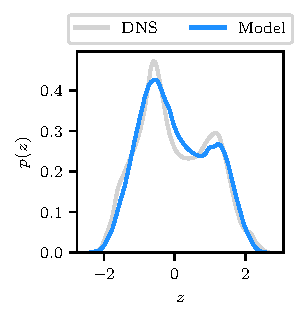
\includegraphics[width=\textwidth]{pdf_comparison_z}
%     \end{overprint}
%   \end{minipage}%
%   \hfill
%   \begin{minipage}{.68\textwidth}
%     \begin{itemize}
%     \item Time-scale distribution is reasonnably well-captured.
%       \begin{itemize}
%       \item[\( \hookrightarrow	\)] Mismatch is \( \mathcal{O}(\Delta t) \).
%       \end{itemize}
      
%       \medskip
      
%     \item Marginal and joint p.d.f.\ are predicted correctly by the model except in the vicinity of \( x = y = 0 \).
%       \begin{itemize}
%       \item[\(	\hookrightarrow	\)] Further physical analyses needed.
%       \end{itemize}
%     \end{itemize}
    
%     \medskip
    
%     \centering
%     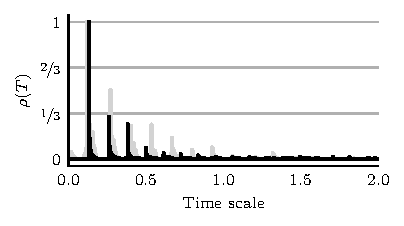
\includegraphics[width=.8\textwidth]{time_scale_distribution_comparison}
%   \end{minipage}
  
%   \vspace{1cm}
% \end{frame}

\begin{frame}[t, c]{Sparse Identification of Nonlinear Dynamics}{Forecasting abilities}
  \begin{minipage}{.48\textwidth}
    \begin{itemize}
    \item The identified model can easily be used for forecasting.
      
      \medskip
      
    \item Some specific regions of phase space are prone to large forecasting errors.
      
      \medskip
      
    \item Forecasts are statistically accurate on the characteristic time-scale \( \tau \).
    \end{itemize}
  \end{minipage}%
  \hfill
  \begin{minipage}{.48\textwidth}
    \begin{overprint}
      \onslide<1>
      \centering
      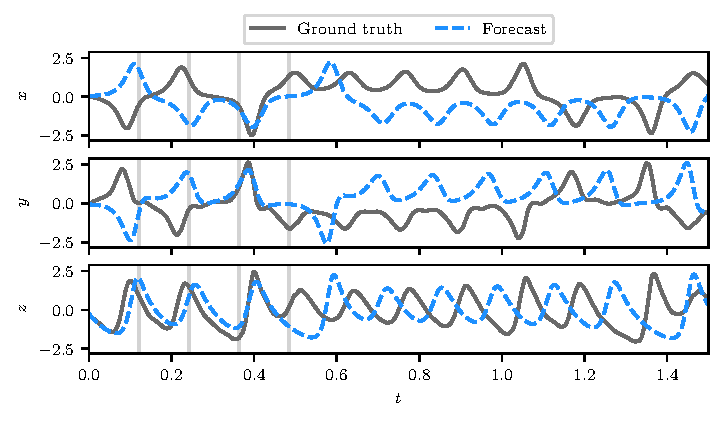
\includegraphics[width=\textwidth]{bad_forecast}
      
      \onslide<2>
      \centering
      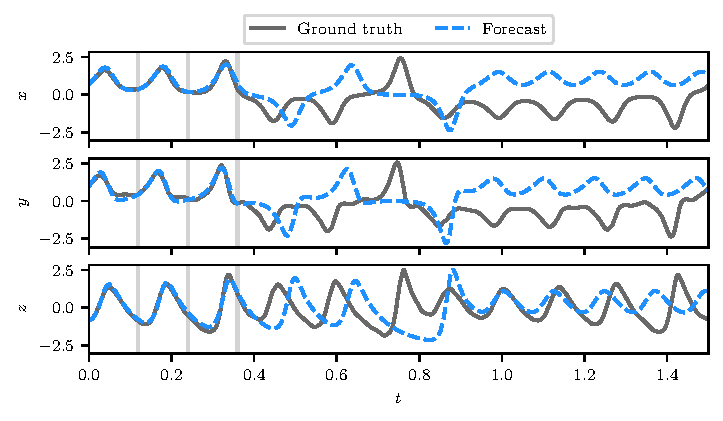
\includegraphics[width=\textwidth]{good_forecast}
      
    \end{overprint}
  \end{minipage}
  
  \vspace{1cm}
\end{frame}

\begin{frame}[t, c]{Sparse Identification of Nonlinear Dynamics}{Eyeball-norm comparison}
  \begin{minipage}{.48\textwidth}
    \centering
    \begin{block}{}
      \centering
      \textbf{Direct numerical simulation}
    \end{block}
    \centering
  
    \movie[width=\textwidth, autostart, loop]{\centering 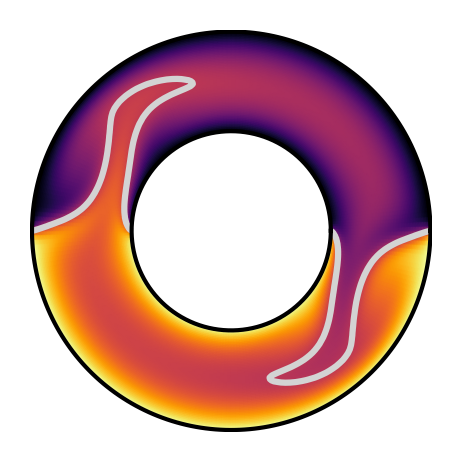
\includegraphics[width=.8\textwidth]{ground_truth}}{imgs/ground_truth.mp4}
  \end{minipage}%
  \hfill
  \begin{minipage}{.48\textwidth}
    \centering
    \begin{block}{}
      \centering
      \textbf{Reduced-order model}
    \end{block}
    \centering
    \movie[width=\textwidth, autostart, loop]{\centering 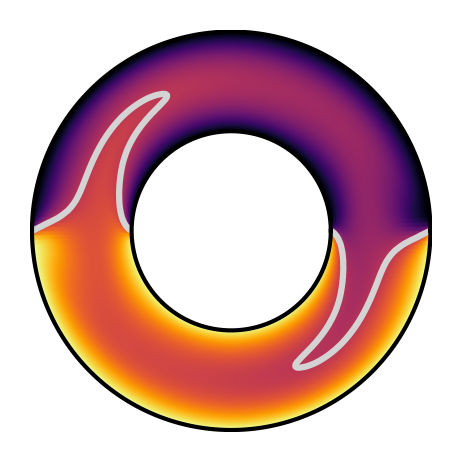
\includegraphics[width=.8\textwidth]{rom_predict}}{imgs/rom_predict.mp4}
  \end{minipage}
  \vspace{1cm}
\end{frame}